% ------------------------------------------------------------------------------------
%                               NOZIONI INTRODUTTIVE
% ------------------------------------------------------------------------------------

\chapter{Nozioni introduttive}

\begin{definition}[OTTIMIZZAZIONE MATEMATICA]
    L'\textbf{ottimizzazione} (o programmazione matematica, PM) è una branca della 
    matematica applicata che studia \textbf{teoria e metodi} per la \textbf{ricerca 
    dei punti di massimo e minimo di una funzione} all'interno di un dominio specificato.
\end{definition}

Per cui, per poter applicare l'ottimizzazione matematica abbiamo bisogno di:
\begin{enumerate}
    \item Un \textbf{insieme di decisioni} (che costituiranno la funzione da ottimizzare).
    \item Poter \textbf{misurare il risultato delle decisioni}.
    \item Poter \textbf{confrontare la "bontà" delle decisioni}.
\end{enumerate}

\section{Modellare la realtà}

In generale, l'ottimizzazione matematica è utilizzata per \textbf{trovare soluzioni ottimali}
a \textbf{problemi reali} (in ambito ingegneristico, industriale, economico-finanziario etc.).

Per prima cosa, abbiamo quindi bisogno di \textbf{creare un modello} che \textbf{descriva
il problema reale}; poi procederemo a \textbf{risolverlo} e, infine, dovremmo
\textbf{interpretare la soluzione} trovata:

\begin{figure}[!ht]
    \centering
    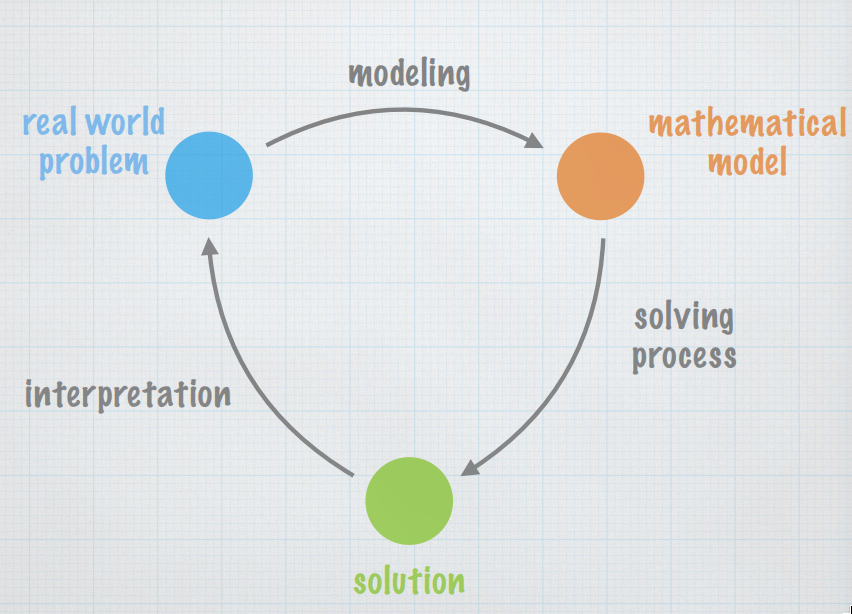
\includegraphics[scale=0.2]{images/01_00_SchemaApplicazioneOttimizzazione.png}
    \caption{Schema di applicazione dell'ottimizzazione matematica}
\end{figure}

\begin{warn}
    La fase di \textbf{interpretazione} è \textbf{spesso sottovalutata}: è
    \textbf{importantissimo} interpretare i risultati per capire
    \textit{cosa rappresentano} e, soprattutto, se \textit{sono compatibili
    con la realtà}.
\end{warn}

\section{Modelli matematici e ottimizzazione}

In generale, i modelli matematici sono delle formulazioni del problema $P$ del tipo:

\begin{definition}[FORMULAZIONE PROBLEMA DI OTTIMIZZAZIONE]
    \[
        \begin{aligned}
            \text{min/max }f(x)& \\ 
            S& \\ 
            x\in D&
        \end{aligned}
    \]
    Dove $f(x)$ è la \textbf{funzione obiettivo} nelle variabili reali $x=(x_{1},\ldots,x_n)$,
    $D=D_{1}\times \ldots \times D_n$ è il dominio di $x$, ed $S$ è un 
    \textbf{insieme finito di vincoli}.
\end{definition}

In genere si considerano problemi di ottimizzazione in cui vogliamo minimizzare la funzione
obiettivo, ma possiamo "convertire" un modello in una o nell'altra forma a piacimento.
Chiariamo ora alcuni dettagli:

\begin{definition}[OTTIMIZZAZIONE DISCRETA]
    Se il dominio $D$ è \textbf{discreto}, si parla di \textbf{ottimizzazione discreta}.
\end{definition}

\begin{definition}[OTTIMIZZAZIONE COMBINATORIA]
    Se il dominio $D$ è \textbf{discreto e finito}, allora si parla di
    \textbf{ottimizzazione combinatoria}.
\end{definition}

\begin{definition}[SOLUZIONE]
    Ogni $x\in D$ è \textbf{soluzione} del problema $P$.
\end{definition}

\begin{definition}[VINCOLO]
    Un vincolo $c\in S$ è una \textbf{funzione} associata ad un
    \textbf{sottoinsieme di variabili} $x_c$, il cui valore può essere
    \textbf{vero} (in tal caso il vincolo è \textbf{soddisfatto}), oppure
    \textbf{falso} (in tal caso il vincolo è \textbf{violato}).
\end{definition}

\begin{definition}[SOLUZIONE AMMISSIBILE]
    Una \textbf{soluzione} che \textbf{rispetti tutti i vincoli} si 
    dice \textbf{ammissibile}.

    L'\textbf{insieme} delle soluzioni ammissibili si indica con $F(P)$.
\end{definition}

\begin{definition}[SOLUZIONE OTTIMA]
    Una soluzione ammissibile $x^*$ si dice \textbf{ottima} se
    \[
        f(x^*) \le f(x) \text{ , } \forall x \in F(P)
    \] 
\end{definition}

Inoltre:

\begin{definition}[PROBLEMA IMPOSSIBILE]
    Un problema di ottimizzazione si dice \textbf{impossibile} (\textit{infeasible})
    se \textbf{non ammette alcuna soluzione ammissibile}, cioè
    $F(P) = \emptyset$
\end{definition}

\begin{definition}[PROBLEMA ILLIMITATO]
    Un problema di ottimizzazione si dice \textbf{illimitato} (\textit{unbounded}) 
    se \textbf{non esiste} alcun \textbf{limite inferiore} a $f(x)$ per $x\in F(P)$.
\end{definition}

\begin{definition}[PROBLEMA RISOLTO]
    Un problema di ottimizzazione si dice \textbf{risolto} quando ne viene
    \textbf{trovata una soluzione ottima} (dimostrando che è tale), oppure 
    quando si \textbf{dimostra che il problema è impossibile o illimitato}.
\end{definition}

E' inoltre importante chiarire il seguente dettaglio:

\begin{warn}[MODELLAZIONE VS RISOLUZIONE]
    In questo corso ci concentreremo sulla fase di \textbf{modellizzazione}.
    Questo perchè:
    \begin{itemize}
        \item Gli \textit{algoritmi risolutivi} sono \textit{incredibilmente 
            complessi} e sono diventati 4-5 ordini di grandezza più
            efficienti nel corso degli ultimi 50 anni; studiarli da zero
            rappresenterebbe solo un handicap.
        \item La fase di modellizzazione è comunque molto importante
            come strumento a disposizione di un ingegnere.
    \end{itemize}
\end{warn}

\section{Paradigmi di ottimizzazione}

Purtroppo, un problema di ottimizzazione \textbf{arbitrario} è \textbf{indecidibile}: è
quindi necessario aggiungere dei vincoli alla \textit{"forma del problema"}.

Chiaramente, imporre dei vincoli ai modelli significa anche \textbf{ridurne l'espressività}
(ovvero possiamo rappresentare fedelmente meno problemi reali); tuttavia esistono due
paradigmi di ottimizzazione che rappresentano un \textbf{buon compromesso} tra \textit{espressività}
e \textit{risolubilità}:
\begin{enumerate}
    \item \textbf{Programmazione Lineare}(PL) - trattata nel corso.
    \item \textbf{Ottimizzazione Convessa} - non trattata nel corso.
\end{enumerate}

\begin{remark}[PROGRAMMAZIONE LINEARE]
    Nella programmazione lineare, la \textbf{funzione obiettivo} ed i \textbf{vincoli}
    sono \textbf{lineari} (duh!). 

    Per quanto stringente possa sembrare questa limitazione,
    moltissimi problemi possono essere modellati in questo modo e, inoltre, si
    tratta di una branca assai matura.
\end{remark}

Di seguito vediamo più nel dettaglio alcuni paradigmi di nostro interesse.

\subsection{Programmazione Lineare}

Un problema di \textbf{programmazione lineare} (LP) consiste nella minimizzazione di 
una \textbf{funzione lineare} soggetta ad un numero finito di \textbf{vincoli lineari}. 
In generale si ha la forma:

\begin{definition}[PROBLEMA DI PROGRAMMAZIONE LINEARE]
    \[
        \begin{aligned}
            \text{min } &c^\top x \\ 
                        &a_i^\top x \sim b_i \text{ , }i=1,\ldots,m \\ 
                        &l_j \le x_j \le u_j \text{ , }j=1,\ldots ,n
        \end{aligned}
    \] 
    Con $\sim \in \{\le , =, \ge \}  $, $l_j\in \mathbb{R} \cup \{-\infty\}  $ 
    e $u_j\in \mathbb{R}\cup \{+\infty\}$.
\end{definition}

Chiariamo ora alcuni dettagli sulle variabili nella definizione:

\begin{remark}[RUOLO DELLE VARIABILI NELLA DEFINIZIONE]
    Le variabili nella definizione hanno i seguenti ruoli:
    \begin{itemize}
        \item Le variabili $x_{1},\ldots,x_n$ compongono il \textbf{vettore delle decisioni} $x$.
        \item $c\in \mathbb{R}^n$ \textit{pesa le variabili} di nostro interesse per
            ottenere la \textit{funzione obiettivo} $c^\top x$.
        \item I vettori $a_i^\top\in \mathbb{R}^n$ \textit{pesano ogni variabile} per
            formalizzare i \textit{vincoli} $i=1,\ldots ,m$.
        \item Il vettore $b=(b_{1},\ldots ,b_m)\in \mathbb{R}^m$ completa la 
            formalizzazione dei vincoli.
    \end{itemize}
\end{remark}

\subsection{Programmazione Lineare Intera}

Un problema di \textbf{programmazione lineare intera}(Mixed Integer Programming) 
consiste nella minimizzazione diuna funzione lineare soggetta ad un numero 
finito di vincoli lineari, con in più il vincolo che \textbf{alcune variabili} 
devono assumere \textbf{valori interi}.

\begin{definition}[PROBLEMA MIP]
    \[
        \begin{aligned}
            \text{min } &c^\top x \\ 
                        &a_i^\top x \sim b_i \text{ , }i=1,\ldots,m \\ 
                        &l_j \le x_j \le u_j \text{ , }j=1,\ldots ,n \\ 
                        &x_j \in \mathbb{Z} \text{ , } \forall j\in J \subseteq N = \{1,\ldots ,n\}  
        \end{aligned}
    \] 
    Con $\sim \in \{\le , =, \ge \}  $, $l_j\in \mathbb{R} \cup \{-\infty\}  $ 
    e $u_j\in \mathbb{R}\cup \{+\infty\}$ come prima.
\end{definition}

Da notare che se $J=N$ si parla di \textit{programmazione lineare intera} \textbf{pura} 
(\textbf{tutte} le variabili sono \textbf{intere}), mentre se $J=\emptyset$ si
ha a che fare con un problema di programmazione lineare classica.

\subsection{Programmazione con Vincoli}

Un problema di \textbf{programmazione con vincoli} è definito da una \textbf{terna} 
$(X, D, C)$, dove $X$ è un insieme di variabili con \textbf{dominio finito} $D$, 
e $C$ è un insieme finito di \textbf{vincoli di natura arbitraria}.

\begin{remark}
    Il paradigma CP è \textbf{molto più libero} nella definizione dei vincoli 
    che si possono usare per modellare un problema. 
    Questo fa si che spesso la modellazione sia più immediata e compatta.

    Di contro, se i vincoli usati \textbf{non} hanno una \textbf{struttura} che 
    \textbf{permetta lo sviluppo di algoritmi efficienti}, la \textbf{capacità di 
    risoluzione} sarà al contrario \textbf{penalizzata}.
\end{remark}

\subsection{Soddisfacibilità booleana}

Un problema di \textbf{soddisfacibilità booleana} è un caso particolare di problema
di \textit{soddisfacibilità}.

\begin{definition}[PROBLEMA DI SODDISFACIBILITA' BOOLEANA]
    \textbf{Tutte le variabili} sono \textbf{booleane} (cioè possono assumere solo i 
    valori \textit{True} o \textit{False} e i \textbf{vincoli} sono un numero 
    finito di \textbf{clausole booleane}.
\end{definition}

Come nel caso LP/MIP, in un problema SAT il \textbf{linguaggio a disposizione} per modellare un
problema di ottimizzazione viene \textbf{notevolmente ristretto}.

\begin{remark}
    Nonostante ciò, molti problemi di notevole importanza pratica, come la 
    \textbf{progettazione di circuiti logici}, possono essere espressi naturalmente 
    con questo paradigma.
\end{remark}
